\usecasebase{Pagamento del conto}
\label{usecase:Pagamento del conto}

\begin{figure}[h]
	\centering
	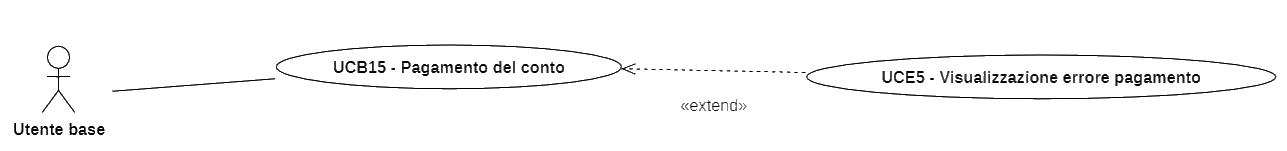
\includegraphics[width=0.9\textwidth]{./uml/UCB15.png} 
	\caption{Pagamento del conto}
	\label{fig:UCB15}
  \end{figure}

\begin{itemize}
	\item \textbf{Attore principale:} Utente base.

	\item \textbf{Precondizione:} L'Utente base ha concluso la divisione del conto (vedi \autoref{usecase:Selezione della modalità di divisione del conto}).

	\item \textbf{Postcondizione:} L'Utente base ha pagato la sua quota.

	\item \textbf{Scenario principale:}
            \begin{enumerate}
                \item Il Sistema mostra la quota che l'Utente base deve pagare;
                \item L'Utene base seleziona la modalità con cui vuole pagare:
                \begin{itemize}
                    \item Pagare in contanti al banco.
                    \item Pagare con la carta al banco.
                    \item Pagare con buoni pasto.
                    \item Pagare in \textit{app}.
                \end{itemize}
				\item L'utente base paga la sua quota.
	      \end{enumerate}

    \item \textbf{Scenario secondario:}
		  \begin{itemize}
			  \item \autoref{usecase:Visualizzazione errore pagamento} Errore pagamento:
				\begin{enumerate}
					\item L'Utente base paga la sua quota attraverso il pagamento in \textit{app};
					\item  Il Sistema mostra un messaggio di errore.
				\end{enumerate}
		  \end{itemize}
\end{itemize}